% =============================================================
% frontmatter-a4.tex — Primeras páginas A4
% Orden: contraportada → presentación → créditos → nota UTN →
%        dedicatoria → mensaje estudiantes → [blanco] → TOC
% =============================================================

% ------------------------------------------------------------------
% PÁGINA 1: Contraportada (imagen a página completa)
% ------------------------------------------------------------------
\newpage
\thispagestyle{empty}
\tikz[remember picture,overlay]
  \node[inner sep=0pt] at (current page.center)
    {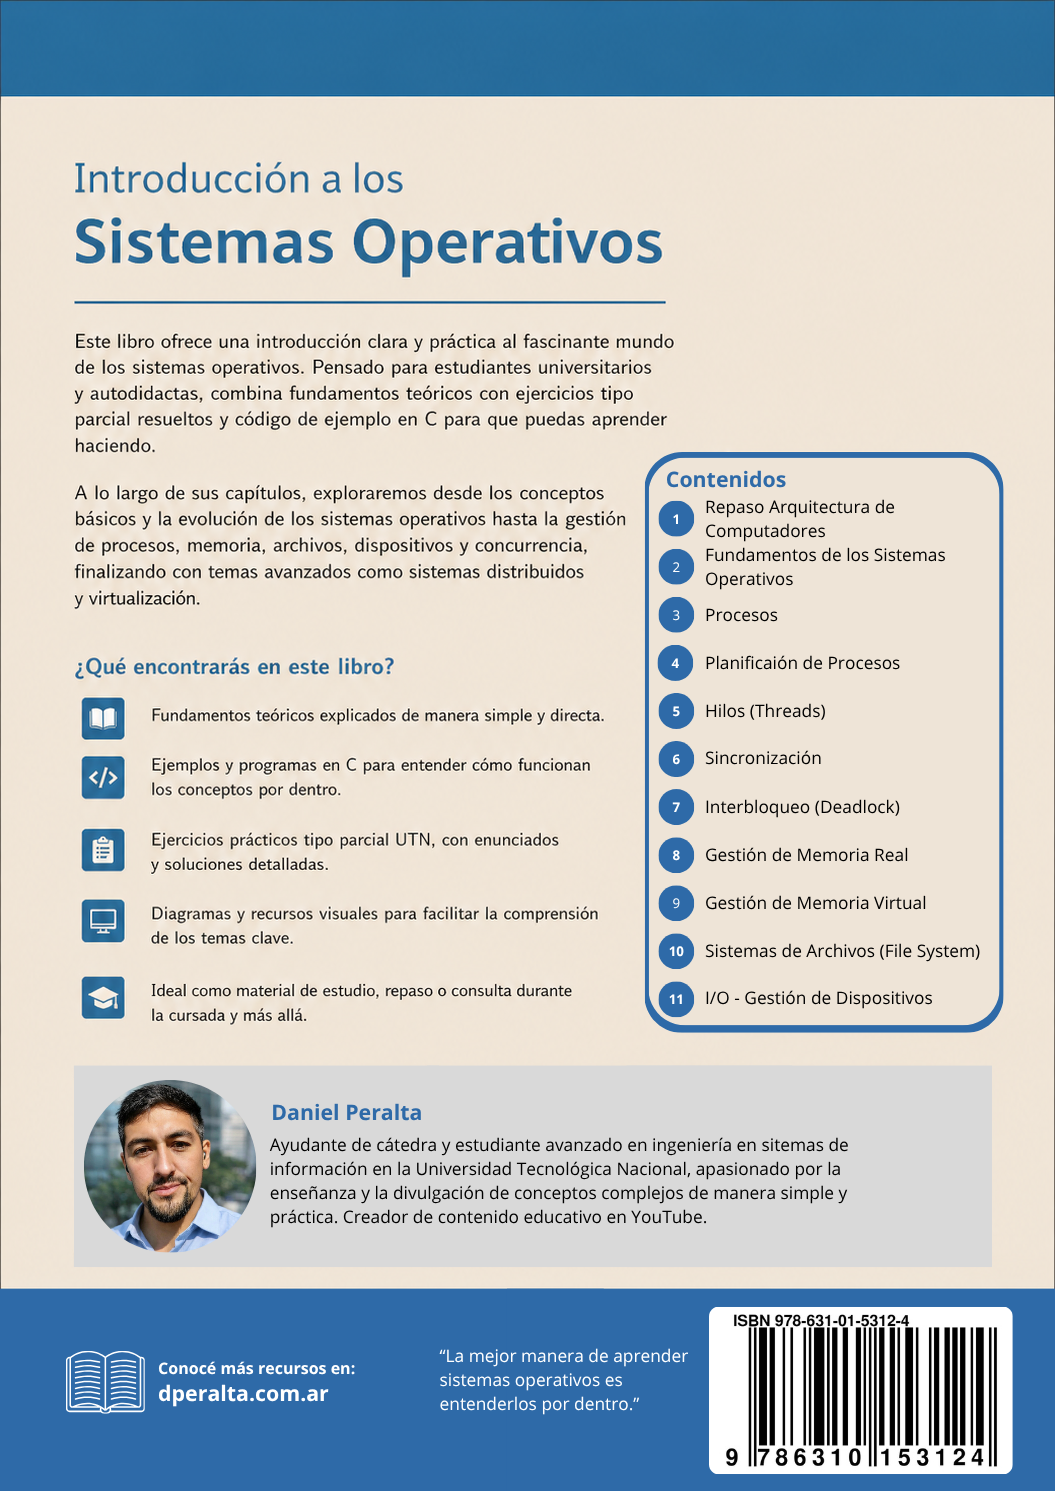
\includegraphics[width=\paperwidth,height=\paperheight]{src/images/contraportada.png}};

% ------------------------------------------------------------------
% PÁGINA 2: Presentación
% ------------------------------------------------------------------
\newpage
\thispagestyle{empty}
\null\vfill
\begin{center}
  {\LARGE\textbf{Introducción a los Sistemas Operativos}}\\[0.8cm]
  {\large\textit{Un enfoque práctico y progresivo para entender}}\\
  {\large\textit{cómo funcionan los sistemas operativos modernos.}}
\end{center}
\vfill
\begin{center}
  \texttt{github.com/dperalta86/Libro-Sistemas-Operativos}\\[0.3em]
  {\small Licencia: Creative Commons BY-SA 4.0}
\end{center}

% ------------------------------------------------------------------
% PÁGINA 3: Créditos e ISBN
% ------------------------------------------------------------------
\newpage
\thispagestyle{empty}
\vspace*{2cm}

\noindent{\large\textbf{Introducción a los Sistemas Operativos}}\\[0.4em]
\noindent\textit{Autor:} Daniel Peralta\\[0.2em]
\noindent\textit{Versión:} 1.0 (Mayo 2026)

\vspace{1.2cm}
\noindent\rule{\textwidth}{0.4pt}
\vspace{0.4cm}

\noindent\textbf{ISBN:} 978-987-12345-67-8\\[0.2em]
\noindent\textbf{Depósito Legal:} N\textordmasculine\ 12345678

\vspace{1cm}

\noindent{\small
\textbf{Licencia:} Creative Commons Atribución-CompartirIgual 4.0.\\
Sos libre de compartir, copiar, distribuir y adaptar este material
bajo los términos de la misma licencia.\\[0.3em]
\texttt{https://creativecommons.org/licenses/by-sa/4.0/}
}

\vspace{0.8cm}

\noindent{\small
\textbf{Código fuente y actualizaciones:}\\[0.2em]
\texttt{github.com/dperalta86/Libro-Sistemas-Operativos}\\[0.2em]
Para reportar erratas o sugerencias, abrí un \textit{issue} en GitHub.
}

\vspace{0.8cm}

\noindent{\small
\textbf{Contacto:}
\texttt{daniel@dperalta.com.ar} ---
\texttt{www.dperalta.com.ar}
}

% ------------------------------------------------------------------
% PÁGINA 4: Nota institucional UTN-FRBA
% ------------------------------------------------------------------
\newpage
\thispagestyle{empty}
\vspace*{3cm}

\begin{center}
  {\small
  Este libro surge en el marco de la materia \textbf{Sistemas Operativos}\\
  de la carrera de Ingeniería en Sistemas de Información\\[0.4em]
  \textbf{Universidad Tecnológica Nacional}\\
  Facultad Regional Buenos Aires (UTN-FRBA)\\[1.5cm]
  \textit{Este es un material independiente creado por un estudiante.\\
  No constituye material oficial de la cátedra ni de la UTN-FRBA.}
  }
\end{center}

% ------------------------------------------------------------------
% PÁGINA 5: Dedicatoria
% ------------------------------------------------------------------
\newpage
\thispagestyle{empty}
\vspace*{5cm}

\begin{center}
  \textit{A mi esposa Cecilia por ser ese equilibrio constante:}\\
  \textit{La que escucha cada idea, incluso las más desordenadas, la que baja todo a tierra cuando hace falta, pero nunca para frenar, sino para ayudarme a seguir mejor.}\\
  \textit{Por acompañarme sin imponer, por sostenerme sin limitar.}\\[0.5em]
  \textit{A mis hijos, Tomás y Jazmín por ser el motor y motivo.}\\
  \textit{Por recordarme, todos los días, para qué vale la pena hacer las cosas bien.}
\end{center}

% ------------------------------------------------------------------
% PÁGINA 6: Mensaje a los Estudiantes
% ------------------------------------------------------------------
\newpage
\thispagestyle{empty}
\vspace*{2cm}

\begin{center}
  {\Large\textit{Mensaje a los Estudiantes}}
\end{center}
\vspace{1.2cm}

\begin{center}
  \begin{minipage}{0.85\textwidth}
    \setlength{\parskip}{0.8em}
    Este material recopila y organiza los conceptos fundamentales de Sistemas Operativos,
    con un enfoque tanto teórico como práctico. Mi intención no es reemplazar las clases
    ni los apuntes, sino ofrecer una guía clara que pueda servir de apoyo al momento
    de estudiar, repasar o preparar exámenes.

    Quiero compartirles también que, al momento de escribir estas páginas,
    todavía sigo siendo estudiante, sigo aprendiendo, cometiendo errores y descubriendo
    nuevas formas de entender estos temas. Por eso, más que un ``manual cerrado'',
    este libro es una invitación a investigar, conocer y aprender.

    Si te resulta útil para aclarar dudas, ordenar ideas o ganar confianza en la materia,
    entonces habrá cumplido su propósito.

    \vspace{0.8cm}
    \centering\textbf{¡Muchos éxitos en la cursada!}
  \end{minipage}
\end{center}

% ------------------------------------------------------------------
% PÁGINA 7: Blanco (para que el índice caiga en página derecha)
% ------------------------------------------------------------------
\newpage
\thispagestyle{empty}
\null
